% Chapter 4

\chapter{RICH Detector}
\label{ch:RICH} % For referencing the chapter elsewhere, use \autoref{ch:name}

%----------------------------------------------------------------------------------------

The particle identification is an important step in the hadron multiplicities extraction.
In the COMPASS spectrometer, it is performed by a large Ring Imaging Cherenkov detector (RICH) capable of separating pions, kaons and protons in a wide momentum range ( $\sim$2 GeV/c to $\sim$60 GeV/c) and an angular overture of 0.01-0.4 radians.

In this chapter the RICH detection principle is presented as well as the description of its main components : the gas and mirror system, the photon detectors, the readout electronics and the data reconstruction.

\section{Cherenkov effect}

When a charged particle is moving through a transparent medium with a speed $v$ greater than the speed of light ($v_{light} = c/n$, $n$ being the medium refractive index), a radiation known as \textit{Cherenkov radiation} is produced by the medium.

\begin{figure}[!h]
  \centering
	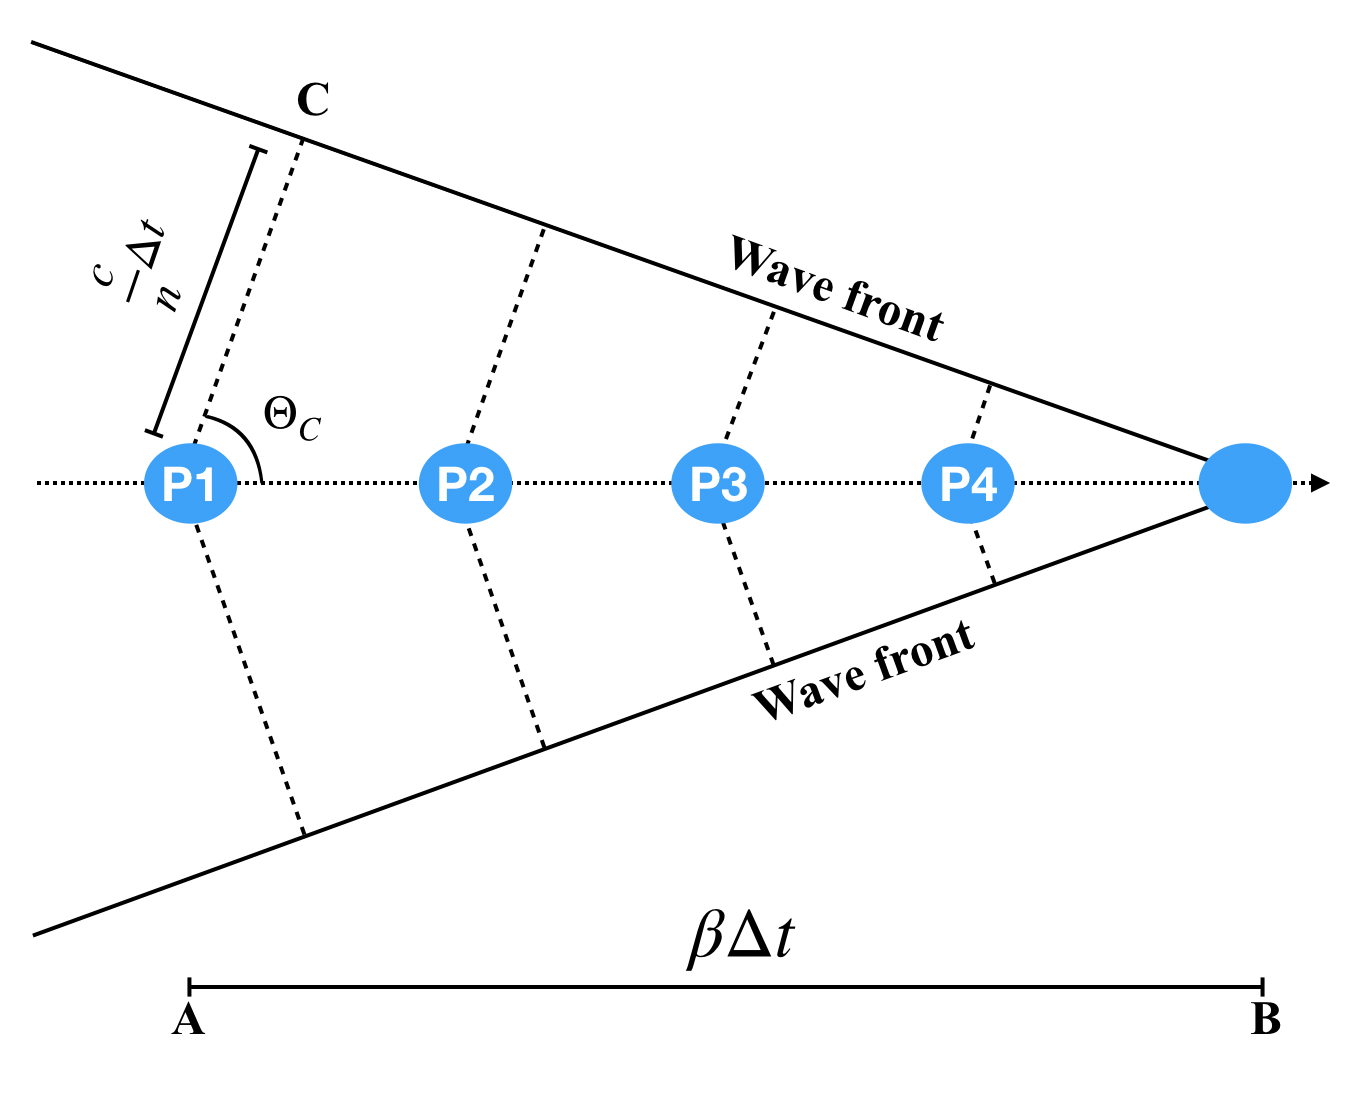
\includegraphics[scale=0.5]{./gfx/CherenkovGeom.png}
	\caption{Cherenkov radiation geometry.}
	\label{pic:CherenkovGeom}
\end{figure}

The Cherenkov radiation produced by a particle with a mass $M_h$ and momentum $p_h$ is emitted only at a particular angle $\Theta_C$ with respect to the particle track (Fig. \ref{pic:CherenkovGeom}).

The coherence between waves (emitted between A and B) is achieved when the particle traverses $\overline{AB}$ at the same time as the radiation travels from A to C. The opening angle $\Theta_C$ is defined geometrically in Eq. \ref{eq:thetaC} with $\beta$ being the particle velocity.

\begin{equation}
  cos\theta_C = \frac{c/n \Delta t}{\beta c \Delta t} = \frac{1}{n\beta}
  \label{eq:thetaC}
\end{equation}

Some limit cases can be devised :
\begin{enumerate}
  \item Threshold limit : if $\beta \leq 1/n$ no Cherenkov radiation will be emitted.
  \item Maximum emission angle : $cos \Theta_C = \frac{1}{n}$ is reached for ultra-relativistic particles ($\beta = 1$).
\end{enumerate}

In order to perform a particle identification with a RICH detector, two variables are needed : $\Theta_C$ and $p_h$. $\Theta_C$ is measured when the photons emitted by the particle is detected. Different techniques can be used to recollect and transport the produced photons where light detectors are placed. The resulting image in the detector plane is a ring with radius propotional to $\Theta_C$. $p_h$ is measured independently by the spectrometer. The particle identification is done by a mass assignment given by :

\begin{equation}
  M_h = p_h \sqrt{n^2 cos^2 \theta_C -1}
\end{equation}

%------------------------------------------------

\section{The COMPASS RICH detector}

The COMPASS RICH detector is designed to distinguish between pions, kaons and protons at high-intensities. The momentum range covers the pion Cherenkov threshold ($\sim$2.67 GeV/c) to $\sim$ 60 GeV/c.

The RICH is a large size detector ($\sim$ 3 x 5 x 6 m$^3$) filled with a gaseous radiator. Two spherical mirror systems reflect the photons into an array of photon detectors (multiwire proportional chambers and multianode photomultipliers tubes), sensitive to a large wavelength range, from visible to far UV, placed outside the spectrometer acceptance, one above and one below the beam line. The whole structure of the detector vessel is built mainly in thin aluminium in order to minimize the material budget.

\subsection{Gas System}

One of the principal elements of a RICH detector is the radiator. At COMPASS it is a gas, C$_4$F$_10$. It has a refractive index of n $\approx$ 1.0015 and a low chromaticity$^(explain in footnote)$ (d$n$/dE $\sim$ 5.10$^{-5}$ eV$^{-1}$). These characteristics allow the particle identification (PID) to be performed in the aforementioned wide momentum range.

The propagation of the Cherenkov photons in the vessel can be affected by the presence of water vapor and oxygen (high UV light absorption cross section). In order to remove these impurities, the gas is constantly circulating and filtered at a constant pressure (1 mbar higher than the atmospheric pressure) in a dedicated gas system\cite{}. The overpressure of the vessel is needed to prevent the air contamination and to avoid mechanical stress to the detector, given its large size. Other circulation system (known as \textit{fast circulation} system) allows a reshuffling of the gas inside the vessel, to avoid stratification that may cause a gradient in the value of the reffractive index from top to bottom.

In order to absorb the photon emitted by the muon beam, a 10 cm diameter pipe filled with helium is positioned inside the vessel on the beam path.

\begin{figure}[!h]
  \centering
	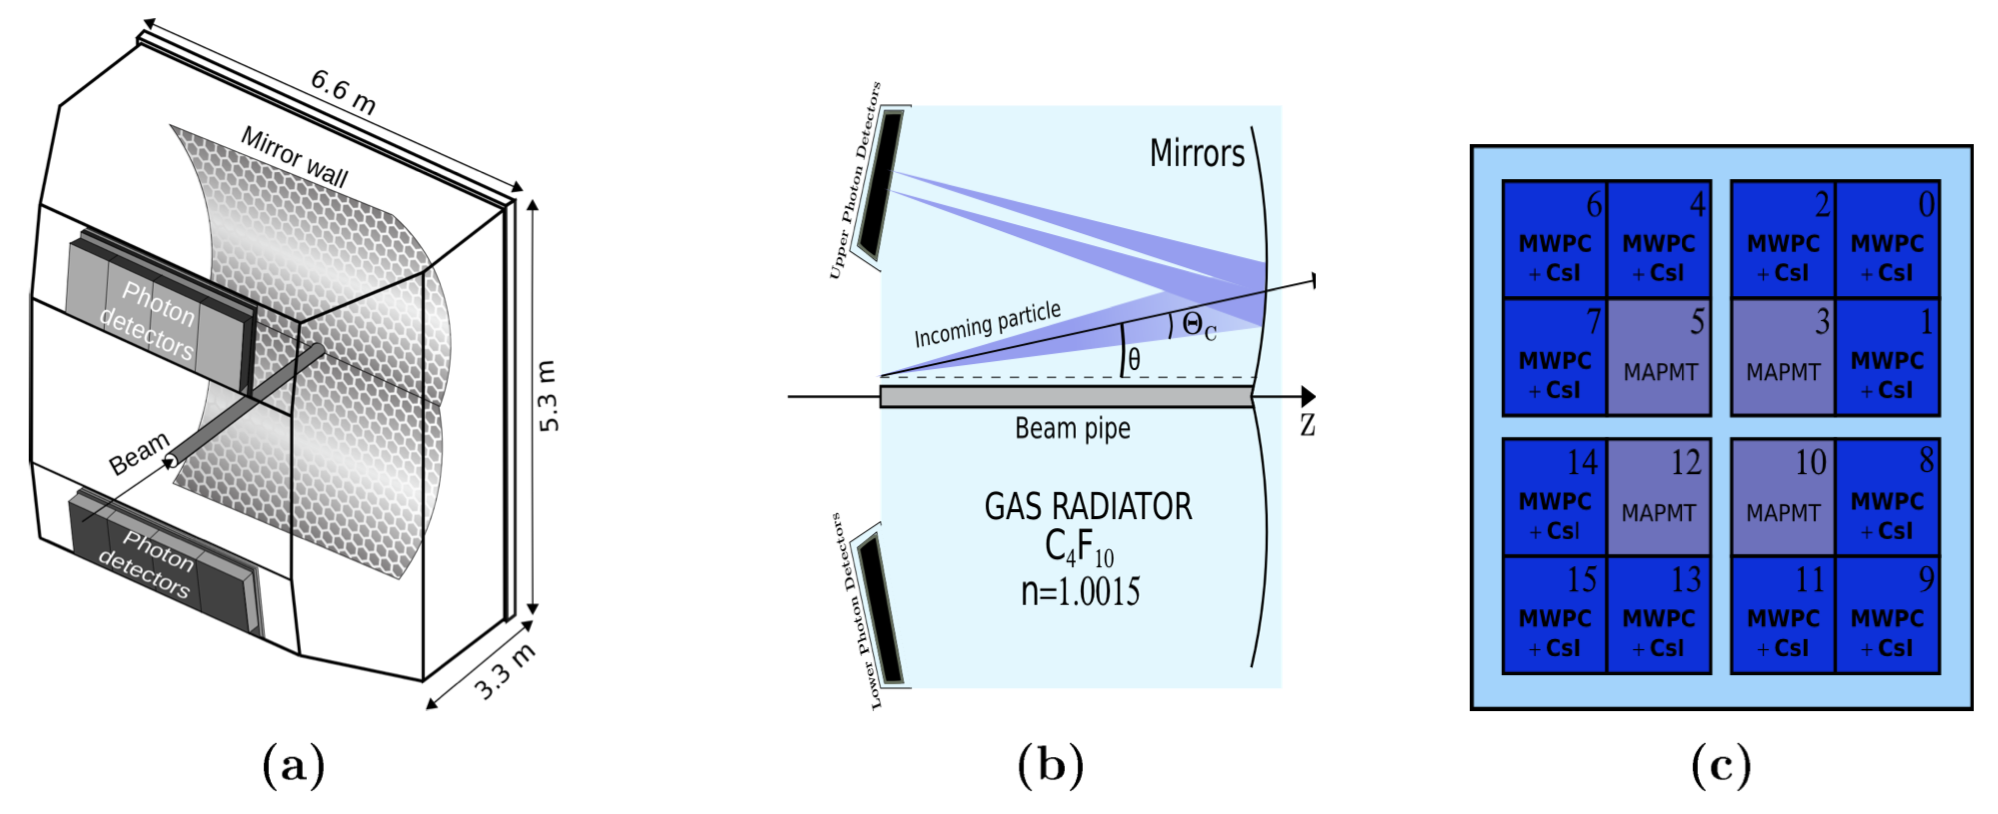
\includegraphics[scale=0.4]{./gfx/RICHview.png}
	\caption{(a) Artistic view of the COMPASS RICH detector. (b) Basic functioning of the RICH detector. (c) Photon detector disposition (not to scale).}
	\label{pic:RICHview}
\end{figure}

\subsection{Mirror System}

The RICH optical system covers an area of $\sim$ 21 m$^2$ and consists of two spherical surfaces, each one containing 58 spherical mirrors of different shapes (34 hexagons and 24 pentagons). The mirror pattern is shown in Fig. \ref{pic:RICHview}. All the mirrors have a reflectance above 80\% in the UV region.

The mirror system has a radius of curvature of 6.6 m. The photon image is focused outside the spectrometer acceptance where the photon detectors are located. As the radius of the curvature is not the same for each mirror ($R$ = 6600 $\pm$ 1\% mm), the reflected image may be slightly blurred. This effect is more pronounced for particles at large angles : this aberration contributes to the dispersion of the photon angle with respect to the angle of emission, which affects the detection resolution.

\begin{figure}[!h]
  \centering
	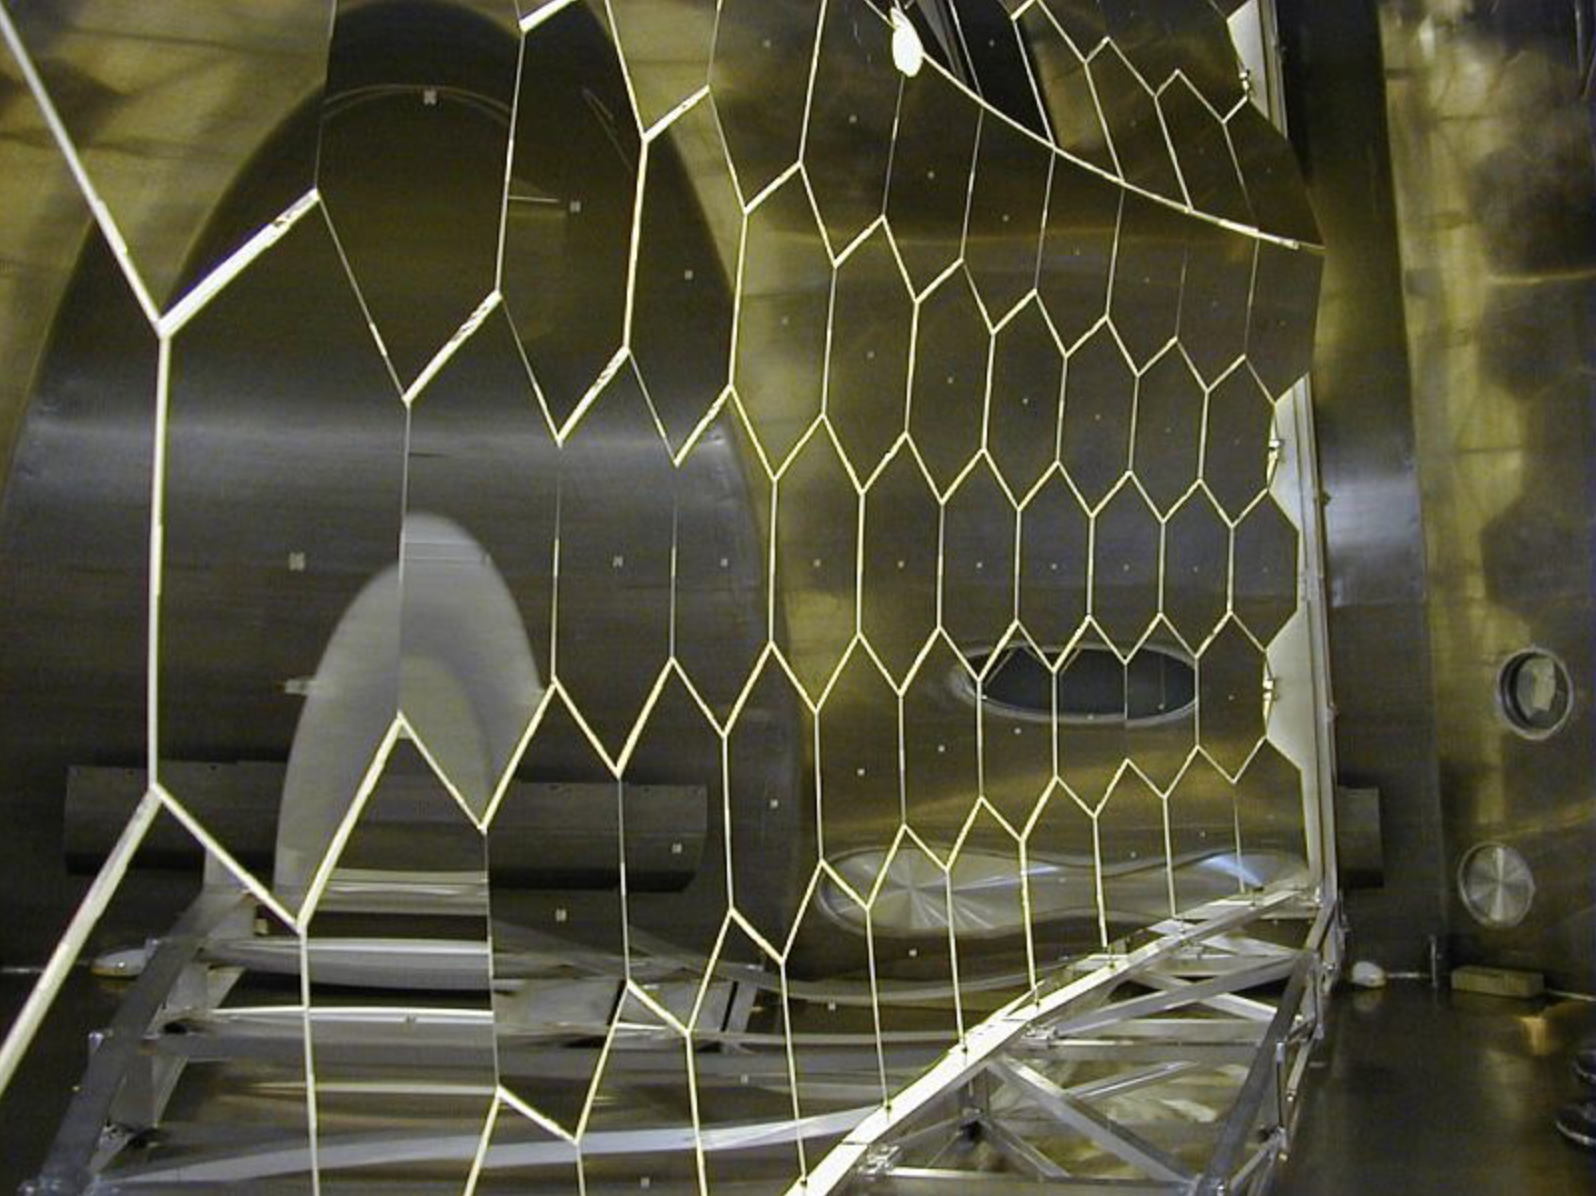
\includegraphics[scale=0.4]{./gfx/RICHmirrors.png}
	\caption{COMPASS RICH detector optical system.}
	\label{pic:RICHmirrors}
\end{figure}

\subsection{Photon Detectors}

The photon detector array consists of two symmetric parts with respect to the beam line, each one is composed by 8 modules. The modules in the external regions are MultiWire Proportional Chambers (MWPC) equipped with solid state CsI photocathodes\cite{}. The central area is composed by MultiAnode Photomultiplier Tubes (MAPMT)\cite{} coupled to individual telescopes of fused silica lenses. The use of two different detector types employing different different photon converters results in the detection of photons in two wavelength regions : < 200 nm for MWPCs and $\sim$ 200 - 650 nm for MAPMT. The low momentum particles are mainly detected by the outer part (MWPC) while the high momentum ones are detected by the central part (MAPMT).

The spherical mirrors will focalize all the photons emitted parallel in the same point. A fortiori the image reflection in the photon detectors will be a ring. An example of a RICH event is shown in Fig. \ref{pic:RICHEvent}.

\begin{figure}[!h]
  \centering
	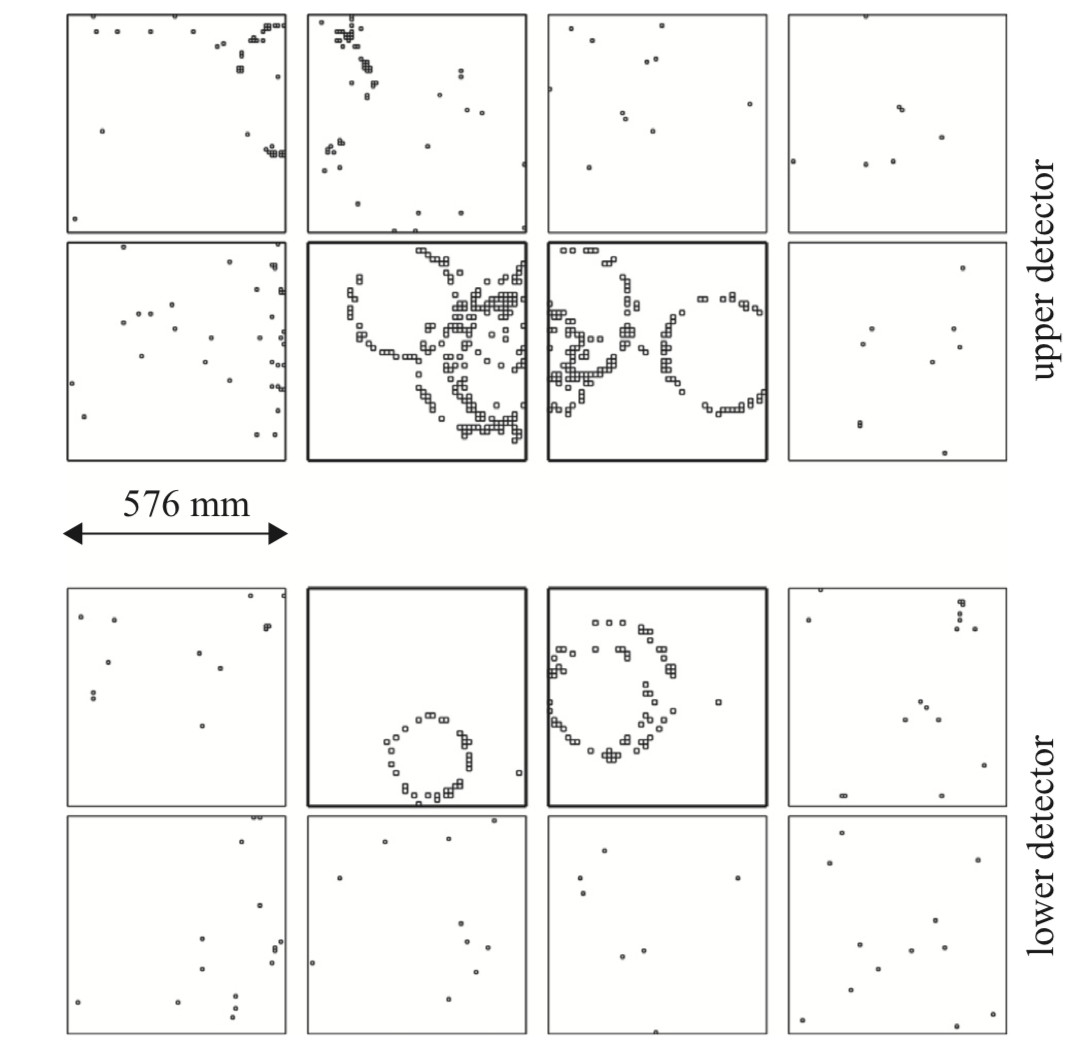
\includegraphics[scale=0.5]{./gfx/RICHEvent.png}
	\caption{An event from the online event display of COMPASS RICHONE; the squares represent the hits with signal amplitudes larger than a threshold, individually set for each channel. Figure taken from \cite{NIM}}
	\label{pic:RICHEvent}
\end{figure}

\subsection{Readout Electronics}

The readout electronics for the central part (MAPMT) consists of three elements : a chip card MAD4, a bus board (Roof) and a DREISAM card. The MAD chip amplifies and discrimates the signal. The latter is then tansported to the chip card DREISAM which functions as a time to digital converter. The signal acquired in a window of 100 ns centered on the time of the trigger is transformed into a temporal information with respect to the absolute time of the experiment with a resolution better than 130 ps. The Roof board acts as a two way bridge to carry the informations from MAD to DREISAM and to deliver to MAD informations about the thresholds. The readout system is free from cable connections to minimize the electrical noise.

From the peripheral area, where events occur at a lower rate with a lower background level, the electronic of the readout system is based on a APV25 chip (128-channel preamplifier /shaper ASIC with analogue pipeline)\cite{}. The chip has an integration time of the signal < 400 ns.

The large number of RICH channels (82944) corresponds to $\sim$ 40\% of the total number of COMPASS electronic channels. To reduce the data flow, empty channels are suppressed at thre front end stage and only the amplitude signals above threshold are read out in local FIFO arrays. Data are then transmitted via optical fibers to the general acquisition system at a rate of 40 MB/s.

\subsection{RICH Event Reconstruction}

RICHONE is a package contained in CORAL software. It is in charge of RICH event reconstruction viz. reconstructs the physical variables from the RICH active pads for each events. The reconstruction is divided in several parts, the first being decoding the data and clustering. Then the reconstruction of the Cherenkov angle for each individual photon is done. It is possible to perform the ring reconstruction which is used for studies on the apparatus. The particle identification (PID) is based on a maximum likelihood calculation. The PID will be explained more thouroughly afterwards.

\subsubsection*{Decoding and clustering}

There are two different types of photon detectors and they have different decoding systems and clustering algorithms. For the MWPCs the analog signal comes from channels having signal (with a three-time sampling of the signal)\cite{}. Since more than one channel fires, a clustering is done. When the pads with the highest pulse height is found, all the adjacent pads with a smaller signal are included in the cluster\cite{}. The mean position of each active pad is evaluated in the cluster, weighting the signal with their maximum pulse height, to determine the center of gravity of the cluster. For the MAPMT signal, decoding is enough to read the time information comming from the PMT that was hit. The probability of having correlated hits in adjacent area being negligible, the MAPMT does not need clustering\cite{}.

The cluster or hit position is used to determine the trajectory of the photon. In addition, the time information coming from the MAPMT is used to reject out-of-time photons while the amplitude information from the MWPC serves to reduce the background both from out-of-time photons and from electronic noise.\cite{}

\subsubsection*{Cherenkov angle and ring reconstruction}

The trajectory of each Cherenkov photon is calculated with respect to the plane containing the particle track and its virtual reflection in the mirror in order to reconstruct $\Theta_C$\cite{}. All the photons emitted by the particles are expected to have the same angle $\Theta_C$ and to be uniformly distributed in $\phi$. The photons emitted by other particles or from background have on the contrary a flat $\Theta_C$ distribution. The emitted photon with the same ($\Theta_C$,$\phi$) pair are reflected on the same point at the focal surface (neglecting any spherical aberration), resulting in a ring image of the photon detector. Since the emission point of the photon along the particle trajectory is not known, the middle point between the detector and the mirror is taken. A good determination of the track trajectory parameters and the momentum of the particle are mandatory in order to extract $\Theta_C$ with good precision.

To characterize the RICH, determining its angular resolution for instance, the ring reconstruction of the emitted photons is needed. The ring reconstruction is based on the search of a peak in the $\Theta_C$ distribution. Small intervals of $\pm$3$\sigma$ ($\sigma$ being the single photon resolution : $\sigma_{MAPMT}$ = 2.0 mrad and $\sigma_{MWPC}$ = 2.5 mrad) on an overall range of 0 to 70 mrad is considered. The interval with the maximum number of entries defines the ring. This procedure associates a ring to each track and in order to reject tracks with only background photons a minimal amount of 4 photons per ring is required\cite{}. The resolution of the Cherenkov angle measurement provided by each single photon as a function of the particle momentum is illustrated in Fig. \ref{pic:RICHRez}. In the high momentum region where the Cherenkov angle saturates the resulting resolution is $\sim$ 1.2 mrad.

\begin{figure}[!h]
  \centering
	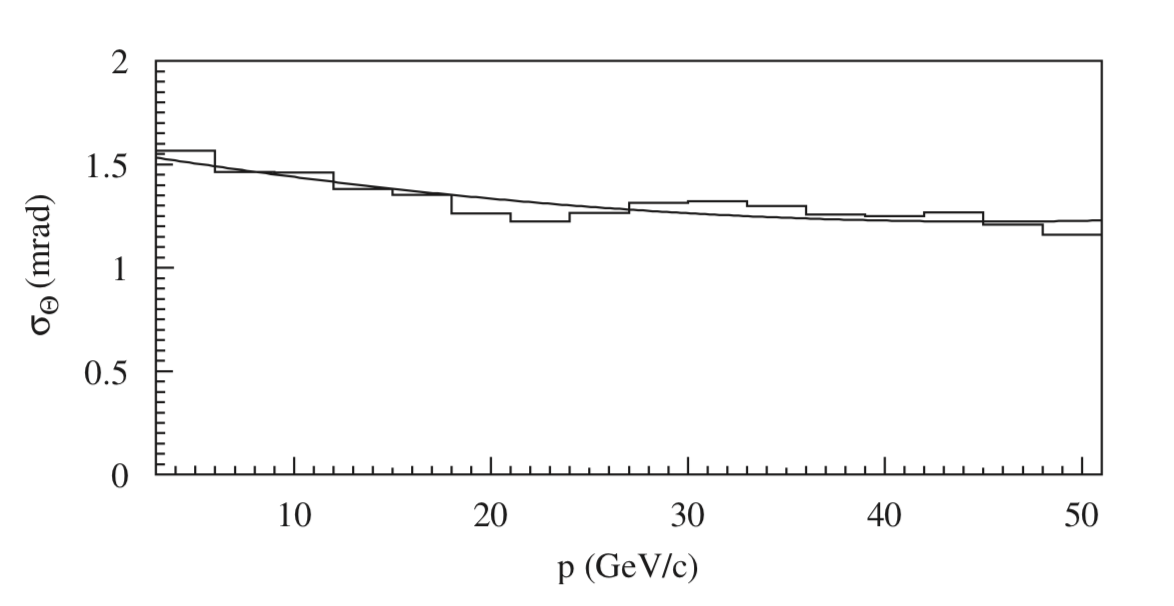
\includegraphics[scale=0.5]{./gfx/RICHRez.png}
	\caption{Resolution of the Cherenkov angle for the reconstructed ring images, provided by each single photon, versus the particle momentum for a sample of identified pions. Figure taken from \cite{NIM}}
	\label{pic:RICHRez}
\end{figure}

\subsubsection*{Mass separation}

For the physical analysis of RICH events, the PHAST software is used. Tha available informations at PHAST is summarized in Tab. \ref{tab:RICHInfos}.

The measured values of $\theta_C$ as a function of $p_h$ for the RICH detector are shown in Fig. \ref{pic:RICH}. In the low momentum region, the RICH detector is only sensitive to electrons, muons and pions. The bands corresponding to kaons and protons start to be visible respectively at $p_h \approx$ 9.45 GeV/c and $p_h \approx$ 17.95 GeV/c. For high momentum values viz. above 40 GeV/c, a saturation of the Cherenkov angle is observed, principally for pions and kaons.

\begin{table}[!h]
  \caption{RICH informations available in PHAST.}
  \label{tab:RICHInfos}
  \centering
  \begin{tabular}{|c|}
    \hline
    $\pi$, $K$, $p$, $e$, $\mu$ and background likelihood \\
    (LH($\pi$), LH($K$), LH($p$), LH($e$), LH($\mu$) and LH($bg$)) \\
    $\pi$, $K$, $p$, $e$, $\mu$ and background likelihood derived\\
    Maximum likelihood angle \\
    $\Theta_{Cj}$, reconstructed ring angle \\
    $N$, number of photons used in $\Theta_C$ reconstruction \\
    $\Theta_{C}$, fitted ring angle \\
    Ring, $\pi$, $K$, $p$, $e$ and $\mu$ $\chi^2$ \\
    Mean ring time for photon in the PMT part \\
    Number of photons per ring in the PMT part \\
    \hline
  \end{tabular}
\end{table}

The final particle identification is performed using likelihood methods and is described in the following chapter.

\begin{figure}[!h]
  \centering
	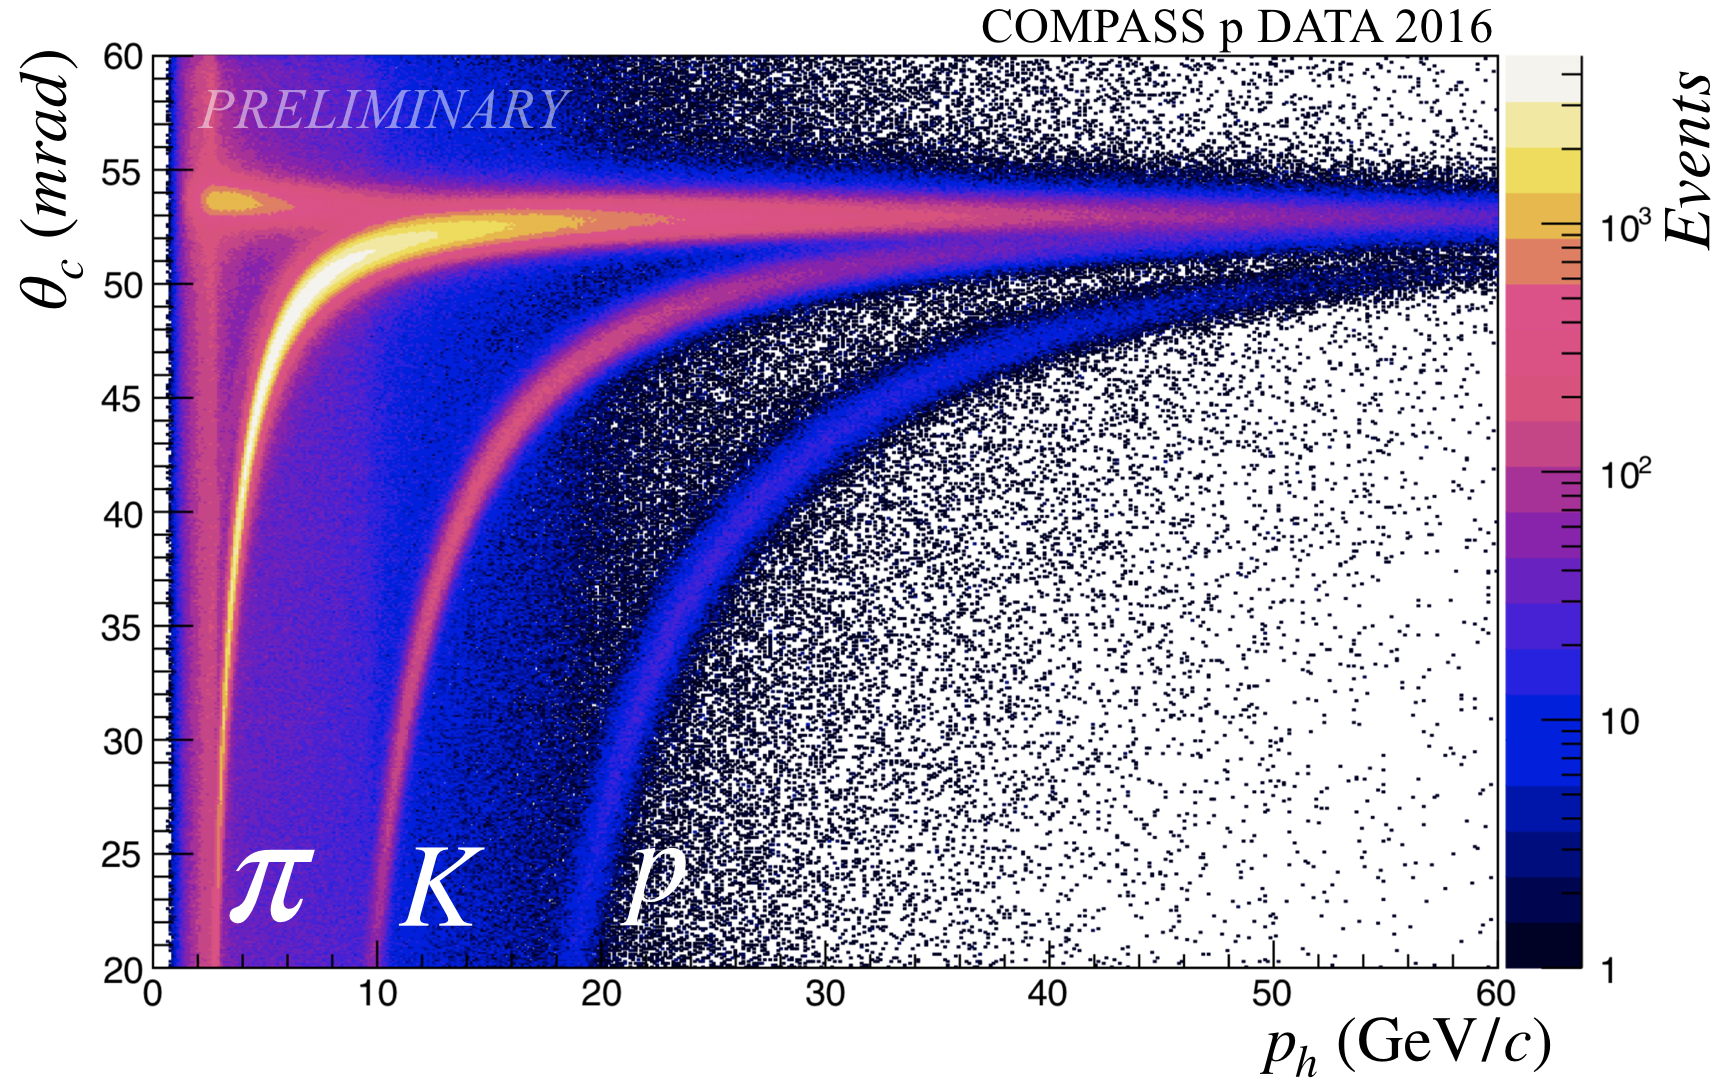
\includegraphics[scale=0.5]{./gfx/RICH.png}
	\caption{Measured Cherenkov angle $\Theta_C$ as a function of $p_h$. $\pi$ threshold $\approx$ 2.67 GeV/c, $K$ threshold $\approx$ 9.45 GeV/c and $p$ threshold $\approx$ 17.95 GeV/c.}
	\label{pic:RICH}
\end{figure}
